\subsubsection{UC 4 - Cambio tema}
\begin{figure}[H]
    \vspace{2em}
    \centering
    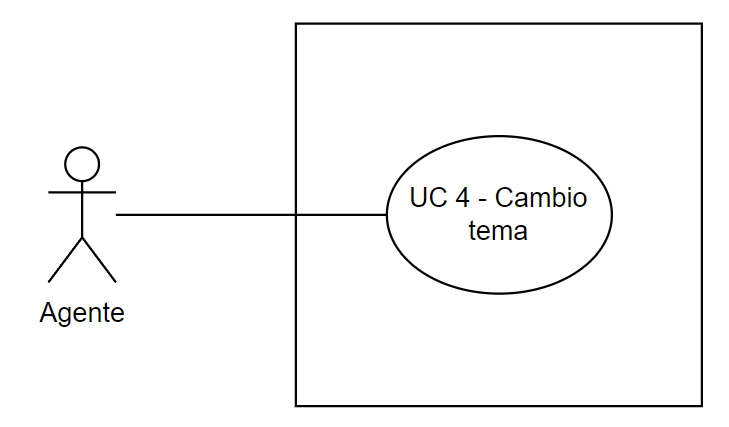
\includegraphics[width=0.75\columnwidth]{img/usecase/UC 4.png}
    \caption{\textit{Use Case} 4: Cambio tema}
    \label{fig:uc_4}
\end{figure}

\begin{usecase}{ 4}{Cambio tema}
    \usecaseactors{Agente.}
    \usecasedesc{L'agente cambia il tema dell'applicazione in chiaro o scuro.}
    \usecasepre{L'agente, dalla \texttt{Homepage Agenti}, cliccando nell'apposito menu il pulsante "Impostazioni", si 
                sposta nella pagina \texttt{Impostazioni}.}
    \usecasepost{L'agente ha cambiato il tema dell'\textit{app}.}
    \usecasescen{
        \begin{itemize}
            \item L'agente si trova nella \texttt{Homepage Agenti};
            \item L'agente preme il pulsante "Impostazioni" dal menu;
            \item L'agente viene spostato nella pagina \texttt{Impostazioni};
            \item L'agente cambia il tema dell'applicazione.
        \end{itemize}}
    \label{uc:uc_4}
\end{usecase}